\documentclass[journal,12pt,twocolumn]{IEEEtran}
%
\usepackage{setspace}
\usepackage{gensymb}
%\doublespacing
\singlespacing
\usepackage{float}
%\usepackage{graphicx}
%\usepackage{amssymb}
%\usepackage{relsize}
\usepackage[cmex10]{amsmath}
%\usepackage{amsthm}
%\interdisplaylinepenalty=2500
%\savesymbol{iint}
%\usepackage{txfonts}
%\restoresymbol{TXF}{iint}
%\usepackage{wasysym}
\usepackage{amsthm}
%\usepackage{iithtlc}
\usepackage{mathrsfs}
\usepackage{txfonts}
\usepackage{stfloats}
\usepackage{bm}
\usepackage{cite}
\usepackage{cases}
\usepackage{subfig}
%\usepackage{xtab}
\usepackage{longtable}
\usepackage{multirow}
%\usepackage{algorithm}
%\usepackage{algpseudocode}
\usepackage{enumitem}
\usepackage{mathtools}
\usepackage{tikz}
\usepackage{circuitikz}
\usepackage{verbatim}
%\usepackage{tfrupee}
\usepackage[breaklinks=true]{hyperref}
%\usepackage{stmaryrd}
\usepackage{tkz-euclide} % loads  TikZ and tkz-base
%\usetkzobj{all}
\usepackage{listings}
    \usepackage{color}                                            %%
    \usepackage{array}                                            %%
    \usepackage{longtable}                                        %%
    \usepackage{calc}                                             %%
    \usepackage{multirow}                                         %%
    \usepackage{hhline}                                           %%
    \usepackage{ifthen}                                           %%
  %optionally (for landscape tables embedded in another document): %%
    \usepackage{lscape}     
\usepackage{multicol}
\usepackage{chngcntr}
%\usepackage{enumerate}

%\usepackage{wasysym}
%\newcounter{MYtempeqncnt}
\DeclareMathOperator*{\Res}{Res}
%\renewcommand{\baselinestretch}{2}
\renewcommand\thesection{\arabic{section}}
\renewcommand\thesubsection{\thesection.\arabic{subsection}}
\renewcommand\thesubsubsection{\thesubsection.\arabic{subsubsection}}

\renewcommand\thesectiondis{\arabic{section}}
\renewcommand\thesubsectiondis{\thesectiondis.\arabic{subsection}}
\renewcommand\thesubsubsectiondis{\thesubsectiondis.\arabic{subsubsection}}

% correct bad hyphenation here
\hyphenation{op-tical net-works semi-conduc-tor}
\def\inputGnumericTable{}                                 %%

\lstset{
%language=C,
frame=single, 
breaklines=true,
columns=fullflexible
}
%\lstset{
%language=tex,
%frame=single, 
%breaklines=true
%}

\begin{document}
%


\newtheorem{theorem}{Theorem}[section]
\newtheorem{problem}{Problem}
\newtheorem{proposition}{Proposition}[section]
\newtheorem{lemma}{Lemma}[section]
\newtheorem{corollary}[theorem]{Corollary}
\newtheorem{example}{Example}[section]
\newtheorem{definition}[problem]{Definition}
%\newtheorem{thm}{Theorem}[section] 
%\newtheorem{defn}[thm]{Definition}
%\newtheorem{algorithm}{Algorithm}[section]
%\newtheorem{cor}{Corollary}
\newcommand{\BEQA}{\begin{eqnarray}}
\newcommand{\EEQA}{\end{eqnarray}}
\newcommand{\define}{\stackrel{\triangle}{=}}

\bibliographystyle{IEEEtran}
%\bibliographystyle{ieeetr}


\providecommand{\mbf}{\mathbf}
\providecommand{\pr}[1]{\ensuremath{\Pr\left(#1\right)}}
\providecommand{\qfunc}[1]{\ensuremath{Q\left(#1\right)}}
\providecommand{\sbrak}[1]{\ensuremath{{}\left[#1\right]}}
\providecommand{\lsbrak}[1]{\ensuremath{{}\left[#1\right.}}
\providecommand{\rsbrak}[1]{\ensuremath{{}\left.#1\right]}}
\providecommand{\brak}[1]{\ensuremath{\left(#1\right)}}
\providecommand{\lbrak}[1]{\ensuremath{\left(#1\right.}}
\providecommand{\rbrak}[1]{\ensuremath{\left.#1\right)}}
\providecommand{\cbrak}[1]{\ensuremath{\left\{#1\right\}}}
\providecommand{\lcbrak}[1]{\ensuremath{\left\{#1\right.}}
\providecommand{\rcbrak}[1]{\ensuremath{\left.#1\right\}}}
\theoremstyle{remark}
\newtheorem{rem}{Remark}
\newcommand{\sgn}{\mathop{\mathrm{sgn}}}
\providecommand{\abs}[1]{\left\vert#1\right\vert}
\providecommand{\res}[1]{\Res\displaylimits_{#1}} 
\providecommand{\norm}[1]{\left\lVert#1\right\rVert}
%\providecommand{\norm}[1]{\lVert#1\rVert}
\providecommand{\mtx}[1]{\mathbf{#1}}
\providecommand{\mean}[1]{E\left[ #1 \right]}
\providecommand{\fourier}{\overset{\mathcal{F}}{ \rightleftharpoons}}
%\providecommand{\hilbert}{\overset{\mathcal{H}}{ \rightleftharpoons}}
\providecommand{\system}{\overset{\mathcal{H}}{ \longleftrightarrow}}
	%\newcommand{\solution}[2]{\textbf{Solution:}{#1}}
\newcommand{\solution}{\noindent \textbf{Solution: }}
\newcommand{\cosec}{\,\text{cosec}\,}
\providecommand{\dec}[2]{\ensuremath{\overset{#1}{\underset{#2}{\gtrless}}}}
\newcommand{\myvec}[1]{\ensuremath{\begin{pmatrix}#1\end{pmatrix}}}
\newcommand{\mydet}[1]{\ensuremath{\begin{vmatrix}#1\end{vmatrix}}}
%\numberwithin{equation}{section}
%\numberwithin{equation}{subsection}
%\numberwithin{problem}{section}
%\numberwithin{definition}{section}
\makeatletter
\@addtoreset{figure}{problem}
\makeatother

\let\StandardTheFigure\thefigure
\let\vec\mathbf
%\renewcommand{\thefigure}{\theproblem.\arabic{figure}}
\renewcommand{\thefigure}{\theproblem}
%\setlist[enumerate,1]{before=\renewcommand\theequation{\theenumi.\arabic{equation}}
%\counterwithin{equation}{enumi}


%\renewcommand{\theequation}{\arabic{subsection}.\arabic{equation}}

\def\putbox#1#2#3{\makebox[0in][l]{\makebox[#1][l]{}\raisebox{\baselineskip}[0in][0in]{\raisebox{#2}[0in][0in]{#3}}}}
     \def\rightbox#1{\makebox[0in][r]{#1}}
     \def\centbox#1{\makebox[0in]{#1}}
     \def\topbox#1{\raisebox{-\baselineskip}[0in][0in]{#1}}
     \def\midbox#1{\raisebox{-0.5\baselineskip}[0in][0in]{#1}}

\title{Convex-Optimization}
\maketitle
\begin{enumerate}
\item There are three food items available, corn, milk, and bread. The table contains,
the cost per serving, the amount of Vitamin A per serving, and the number of
calories per serving for each food item. Also, there are restrictions on the total
number of calories (between 2000 and 2250) and the total amount of Vitamin A
(between 5000 and 50,000) intake in the diet.The goal of the diet problem is to
select a set of food items that will satisfy a set of daily nutritional requirement
at minimum cost. The maximum number of servings is 10 per food item. Table 1 shows all the content per serving.\\
\begin{table}[H]
 \centering
 \resizebox{\columnwidth}{!}{
 \begin{tabular}{ |c|c|c|c| } 
 \hline
 Food & Cost & Vitamin A  & calories  \\
 \hline
Corn & 0.18 USD & 107 & 72\\
 \hline
 Milk & 0.23 USD & 500 & 121\\
 \hline
 Wheat Bread & 0.05 USD &0 &65\\
 \hline
\end{tabular}}
 \caption{}
 \end{table}
\solution\\ 
Consider,\\
\begin{table}[H]
 \centering
 \resizebox{\columnwidth}{!}{
 \begin{tabular}{ |c|c|c| } 
 \hline
 \textbf{Description} & \textbf{Parameter} & \textbf{Value}  \\
 \hline
Cost per serving & $\vec{c}$ & $\myvec{0.18\\0.23\\0.05}$ \\
 \hline
 Vitamin A per serving &$ \vec{v} $&$ \myvec{107\\500\\0}$\\ 
 \hline
 Calories per serving & $\vec{u}$ &$\myvec{72\\121\\65}$\\ 
 \hline
 No. of servings &$\vec{x}$ &$ \myvec{x\\y\\z}$\\
 \hline
\end{tabular}}
 \caption{}
 \end{table}
Objective function 
\begin{align}
z = \min_\vec{x} \vec{c}^T\vec{x}
\end{align}
Constraints
\begin{align}
&5000 \leq 107x+500y+0z \leq 50000\\
&2000 \leq 72x+121y+65z \leq 2250\\
&0 \leq x \leq 10\\
&0 \leq y \leq 10\\
&0 \leq z \leq 10
\end{align}
Writing all the constraints in the matrix form
\begin{align}
&\vec{p}\vec{x} = \vec{q}\\
&\myvec{107&500&0\\-107&-500&0\\72&121&65\\-72&-121&-65\\1&0&0\\0&1&0\\0&0&1\\-1&0&0\\0&-1&0\\0&0&-1}\vec{x}=\myvec{50000\\ -5000\\ 2250\\ -2000\\ 10\\ 10\\ 10\\ 0\\ 0\\ 0}
\end{align}
By providing the objective function and constraints to cvxpy, we get the optimal cost (z) and optimal no.of servings $(\vec{x})$.\\
cvxpy code,
\begin{lstlisting}
https://github.com/gadepall/EE5606-optimization/codes/opt_1.py
\end{lstlisting}
From cvxpy, we get
\begin{align}
& z= 3.16  \text{USD}\\
& \vec{x} = \myvec{2\\10\\10}
\end{align}
\item Funding an expense stream. Your task is to fund an expense stream over n time periods.
We consider an expense stream $\vec{e}$ $\epsilon$ $R^n$, so that $e_t$ is our expenditure at time t.
One possibility for funding the expense stream is through our bank account. At time
period t, the account has balance $b_t$ and we withdraw an amount $w_t$. The value of our
bank account accumulates with an interest rate $\rho$ per time period, less withdrawals
\begin{align}
b_{t+1} = (1+ \rho)b_t - w_t \nonumber
\end{align}
We assume the account value must be nonnegative, so that $b_t \geq$ 0 for all t.
We can also use other investments to fund our expense stream, which we purchase at
the initial time period t = 1, and which pay out over the n time periods. The amount
each investment type pays out over the n time periods is given by the payout matrix
$\vec{P}$, defined so that $P_{tj}$ is the amount investment type j pays out at time period t per
dollar invested. There are m investment types, and we purchase $x_j \geq$ 0 dollars of
investment type j. In time period t, the total payout of all investments purchased is
therefore given by $({P x})_{t}$.
In each time period, the sum of the withdrawals and the investment payouts must
cover the expense stream, so that
\begin{align}
w_t + ({P x})_t \geq e_t \nonumber
\end{align}
for all t = 1, . . . , n.
The total amount we invest to fund the expense stream is the sum of the initial account
balance, and the sum total of the investments purchased: $b_1 + 1^T \vec{x}$.\\
Using the data in \textbf{expense stream data.$^*$,}Show that the minimum initial investment that funds the expense stream can be
found by solving a convex optimization problem.\\
\solution\\
Consider,
\begin{table}[H]
 \centering
 \resizebox{\columnwidth}{!}{
 \renewcommand{\arraystretch}{2}
 \begin{tabular}{ |c|c|c| } 
 \hline
 \textbf{Description} & \textbf{Parameter} & \textbf{Value}  \\
 \hline
Payout Matrix & $\vec{P}_{nxm} $ & from expense stream data.py  \\
 \hline
 expense stream & $\vec{e}_{nx1}$ &from expense stream data.py  \\ 
 \hline
 Interest rate & $\rho$ &from expense stream data.py \\ 
 \hline
 No. of investments & m &from expense stream data.py \\
 \hline
 Time period & n &from expense stream data.py \\
 \hline
  Present Bank balance & $\vec{b}_{n x 1}$ & $?$ \\
 \hline
Bank withdrawals & $\vec{w}_{n x 1}$ & $?$ \\
 \hline
Investments purchased & $\vec{x}_{m x 1}$ & $?$ \\
 \hline
Total payable for investments purchaced & $\vec{Px}_{n x 1}$ & ? \\
 \hline
\end{tabular}
\renewcommand{\arraystretch}{1}}
 \caption{}
 \end{table}
Given to minimize the inital investment.\\
Objective Function,
\begin{align}
Z = \min_{b1,\vec{x}} b_1 + 1^T \vec{x}
\end{align}
Constraints,
\begin{align}
&\vec{b} \succeq 0   \\
&\vec{x} \succeq 0 \\
&\vec{w} + \vec{P x} \succeq \vec{e} \\
&b_{t+1} = (1+ \rho)b_t - w_t .
\end{align}
Solution of the above objective function with the constraints is obtained by CVXPY.\\
CVXPY code, 
\begin{lstlisting}
https://github.com/gadepall/EE5606-optimization/codes/opt_2.py
\end{lstlisting}
\begin{lstlisting}
https://github.com/gadepall/EE5606-optimization/codes/expense_stream _data.py
\end{lstlisting}
The optimal initial investment Z = 177.51
\item We are tasked with designing a box shaped with width $w$, height $h$, and depth $d$. We are given that the total wall area is at most 200 square units, the total floor area is at most 60 square units, and the aspect ratios (h/w ans d/w) are at least 0.8 and at most 1.2. Formulate an optimization program to solve for the dimensions h,w and d that results in a box of the largest possible volume, and implement in CVXPY.\\
\solution\\
Given 
\begin{table}[H]
 \centering
 \resizebox{\columnwidth}{!}{
 \begin{tabular}{ |c|c|c| } 
 \hline
 \textbf{Description} & \textbf{Parameter} & \textbf{Value}  \\
 \hline
 Width & w & ? \\
 \hline
Height & h & ? \\
 \hline
 Depth &d & ? \\
 \hline
 Volume & v & ? \\
 \hline
 Wall area  & 2(wh+hd) & $\leq$ 200 \\
 \hline
 Floor area  & dw &$ \leq$ 60 \\
 \hline
 Aspect ratio = h/w and d/w & $a_1$ and $a_2$ & $\leq$ 1.2 and $\geq $0.8 \\
 \hline
\end{tabular}}
 \caption{}
 \end{table}

Let $\vec{w}$ be the optimization variables vector.
\begin{align}
\vec{w} = \myvec{w\\h\\d}
\end{align}
Objective is to maximize the volume of the box. \\
\begin{align}
{v=whd} \nonumber
\end{align}

Objective function is defined as,
\begin{align}
&z= \max_{w,h,d} (whd)
\end{align}
constraints are,
\begin{align}
& {wh\leq 200}\\
&{ dw \leq 60}\\
&{0.8\leq a_1\leq 1.2}\\
&{0.8\leq a_2 \leq 1.2}
\end{align}
Writing constraints in the matrix form, 
\begin{align}
&\vec{w}^\text{T}\vec{P_1}\vec{w} \leq q_1\\
& \myvec{w&h&d}\myvec{0&1&0\\0&0&0\\0&1&0}\myvec{w\\h\\d} \leq 100\\
&\vec{w}^\text{T}\vec{P_2}\vec{w} \leq q_2\\
& \myvec{w&h&d}\myvec{0&0&1\\0&0&0\\0&0&0}\myvec{w\\h\\d} \leq 60\\
&\vec{P_3}\vec{w}\leq \vec{q_3}\\
&\myvec{-0.8&-1&0\\1&-1.2&0\\-0.8&0&-1\\1&0&-1.2} \myvec{w\\h\\d} \leq \myvec{0\\0\\0}
 \end{align}
Solving the objective function and constrains by cvxpy.\\
cvxpy code,
\begin{lstlisting}
https://github.com/gadepall/EE5606-optimization/codes/opt_3.py
\end{lstlisting}
The maximum optimum value is 387.29 cubic units.\\
Optimum w = 7.74, h = 6.45, d = 7.74 units. 
\item A fictional company AccessApple  \&  Co. produces three types of covers for Apple products:
one for iPod, one for iPad, and another for iPhone. The company's production facilities are
such that if we devote the entire production to iPod covers, we can produce 6000 of them
in a day. If we devote the entire production to iPhone covers or iPad covers, we can
produce 5000 or 3000 of them, respectively, in one day.
The production schedule is one work week of 5 working days, and the week's production
must be stored before distribution. Storing 1000 iPod covers (packaging included) takes up
40 cubic feet of space. Storing 1000 iPhone covers (packaging included) takes up 45 cubic
feet of space, and storing 1000 iPad covers (packaging included) takes up 210 cubic feet of
space. The total storage space available is 6000 cubic feet.
Due to a commercial agreement, AccessApple \& Co. has to deliver at least 5000 iPod
covers, and 4000 iPad covers per week in order to strengthen the products’ diffusion.
The marketing department estimates that the weekly demand for iPod covers, iPhone, and
iPad covers does not exceed 10000 and 15000 , and 8000 units, respectively. Therefore the
company does not want to produce more than these numbers.
Finally, the net profits in USD for each iPod cover, iPhone cover, and iPad cover are USD 4,
USD 6 and USD 10 respectively.
The aim is to determine a weekly production schedule that maximizes the total net
profit. \\

\solution \\
Consider,\\
x= proportion of time devoted each day to iPod cover production,\\
y= proportion of time devoted each day to iPhone cover production,\\
z= proportion of time devoted each day to iPad cover production.\\
\begin{table}[H]
 \centering
 \resizebox{\columnwidth}{!}{
 \begin{tabular}{ |c|c|c| } 
 \hline
 \textbf{Description} & \textbf{Parameter} & \textbf{Value}  \\
 \hline
 Proportion of time devoted & $\vec{x}$ & $\myvec{x\\y\\z}$  \\ 
 \hline
Production per day & $\vec{p}_p $ & $\myvec{6,000\\ 5,000\\ 3,000} $ \\
 \hline
 Storage per 1000 units & $\vec{s}$ & $\myvec{40\\ 45\\ 210} $ \\ 
 \hline
 minium requirement & $\vec{m}_r$ & $\myvec{5,000\\0\\4,000} $  \\
 \hline
 Maximum Production & $\vec{m}_p$ & $\myvec{10,000\\15,000\\8,000}$ \\
 \hline
 Profit & $\vec{p}$ & $\myvec{4\\6\\10} $ \\
 \hline
 profit for week  & $\vec{c}$ & $\myvec{120000\\15000\\15000} $ \\
 \hline
\end{tabular}}
 \caption{}
 \end{table}
 The elements of $ \vec{c}$ are the product of production per day, profit and no.of workings day in a week for ipod, iphone and ipad respectively.\\
Objective function,
\begin{align}
z = \max_\vec{x} \vec{c}^T\vec{x}\\
z = \min_\vec{x} (- \vec{c}^T\vec{x})
\end{align}
constrains,
\begin{align}
x+y+z \leq 1\\
1200x+1125y+3150 \leq 6000\\
30,0000x \geq 5000\\
15,000z \geq 4000\\
30,000x \leq 10,000\\
25,000y \leq 15,000\\
15,000z \leq 8,000\\
\vec{x}\succeq 0
\end{align}
Putting all the constrains in the form$\vec{P}\vec{x}=\vec{q}$,
\begin{align}
\myvec{1&1&1\\1200&1125&3150\\-30,000&0&0\\0&0&-15,000\\30,000&0&0\\0&25,000&0\\0&0&15,000\\-1&0&0\\0&-1&0\\0&0&-1}\vec{x} \leq \myvec{1\\6,000\\-5,000\\-4,000\\10,000\\15,000\\8,000\\0\\0\\0}
\end{align}
Solving the objective function and constrains by cvxpy.\\
cvxpy code,
\begin{lstlisting}
https://github.com/gadepall/EE5606-optimization/codes/opt_4.py
\end{lstlisting}
The maximum weekly profit= 1,45,000 USD.\\
Optimum time devoted, $\vec{x} = \myvec{0.1667\\ 0.4129\\ 0.4203}$.
\item Decomposing a PV array output time series: We are given a time series  $\vec{p} \in \Re_+^T $ that gives the output power of photo-voltaic array in 5 minutes intervals, over T = 2016 periods, given in pv output data.*. In this problem you will use convex optimization to decompose the time series into three components:
\begin{itemize}
\item The clear sky output $\vec{c} \in \Re_+^T $, a smmoth daily-periodic component, which gives what the PV output would have been without clouds. This signal is 24-hour-periodic,  i,e., $c_{t+288} = c_t$ for t = 1,2, ...... T-288. (The clear sky output is zero at night, but we will not use this prior information in our decomposition method).
\item A weather shading loss component $\vec{s} \in \Re_+^T $, which gives the loss of power due to clouds. This component satisfies $0 \succeq \vec{s} \succeq \vec{c}$, can change rapidly, and is not periodic.
\item A residual $\vec{s} \in \Re_+^T $, which accounts for measurements error, anomalies, and other errors.
 \end{itemize}  
 These components sastisfy $ \vec{p}=\vec{c}-\vec{s}+\vec{r}$\\
 We will assume that the average absolute value of the residual is no more than 4.\\
 Smoothness of  $\vec{c}$ is measured by its Laplacian,
 \begin{align}
 \mathcal{L}(c) = (c_1 - c_2)^2 + ..+(c_{287} -c_{288})^2 + (c_{288} - c_{1})^2  \nonumber
 \end{align}
 We will choose $\vec{c} ,\vec{s}  \text{ and }  \vec{r}$ by minimizing $\mathcal{L}(c) + \lambda1^T\vec{s} $ subject to the constraints described above, where $\lambda$ is a positive parameter, that we take to be one.\\
 Solve this problem, and plot the resulting $\vec{c} ,\vec{s}, \vec{r} \text{ and } \vec{p}$ on separate plots. Give the average values of c, s and p and the average value of r (which should be 4).\\
\solution \\
Consider,
\begin{table}[H]
 \centering
 \resizebox{\columnwidth}{!}{
 \begin{tabular}{ |c|c|c| } 
 \hline
 \textbf{Description} & \textbf{Parameter} & \textbf{Value}  \\
 \hline
 PV array output & $\vec{p}$ & pv output data.py  \\ 
 \hline
Clear sky output & $\vec{c}$ & $? $ \\
 \hline
 Weather shading loss component &$\vec{s}$ & $? $ \\ 
 \hline
residual & $\vec{r}$ & $? $  \\
 \hline
 Total Period & T  & 2016   \\
 \hline
  Samples  & N  & 288   \\
 \hline
 \end{tabular}}
 \caption{}
 \end{table}
 Objective function,
  \begin{align}
 z= \min_{\vec{s},\vec{c}} \mathcal{L}(c) + \lambda1^T\vec{s}
 \end{align}
 Writing the objective function in terms of matrices,\\
 Let $\vec{c}_1$ is a vector of size 288 X 1, first 288 elements of vector$\vec{c}$
 \begin{align}
 &(c_1 - c_2)^2 + ..+(c_{287} -c_{288})^2 + (c_{288} - c_{1})^2 = \nonumber \\
 &[\vec{c_1 - A c_1}]^\text{T} [\vec{c_1 - A c_1}]	\\
 &\vec{A} = \myvec{0&1&0&.&.&.&0\\.&.&.&.&.&.&.&\\.&.&.&.&.&.&.&\\0&0&0&.&.&.&1\\1&0&0&.&.&.&0}
\end{align} 
Objective function can be modified as,
\begin{align}
 z= \min_{\vec{s},\vec{c}} [\vec{c_1 - A c_1}]^\text{T} [\vec{c_1 - A c_1}] + \lambda1^T\vec{s}
\end{align}
Constraints are listed below,
\begin{align}
&0 \preceq \vec{s} \preceq \vec{c}\\
& \vec{p}=\vec{c}-\vec{s}+\vec{r}\\
& c_{t+288} = c_t\\
& (\|\vec{r}\|_1)/\text{T}
\end{align}
Solving the objective and constraints by CVXPY.\\
CVXPY code,
\begin{lstlisting}
https://github.com/gadepall/EE5606-optimization/codes/opt_5.py
\end{lstlisting}
From cvxpy, 
\begin{align}
& z= 98131.26\\
&\text{avg of c} = 529.51\\
& \text{avg of s} =4.47 \\
& \text{avg of p} = 529.03\\
& \text{absolute avg of r} = 3.99
\end{align}
We get the plots for  $\vec{c} ,\vec{s}  \text{ and }  \vec{r}$ .
\begin{figure}[H]
	\centering
    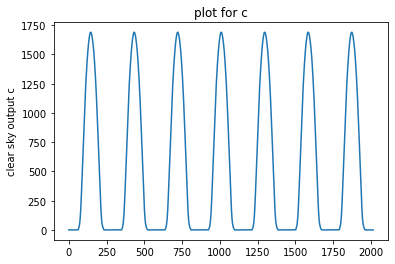
\includegraphics[width=\columnwidth]{c.png}
    \caption{Clear sky plot}
    \label{}
\end{figure}
\begin{figure}[H]
	\centering
    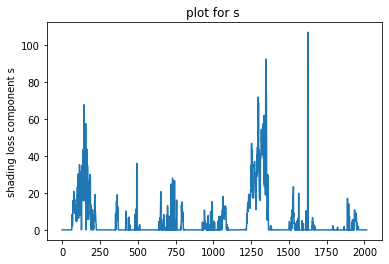
\includegraphics[width=\columnwidth]{s.png}
    \caption{shading loss plot}
    \label{}
\end{figure}
\begin{figure}[H]
	\centering
    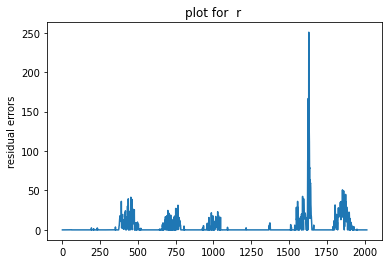
\includegraphics[width=\columnwidth]{r.png}
    \caption{residual plot}
    \label{}
\end{figure}
\begin{figure}[H]
	\centering
    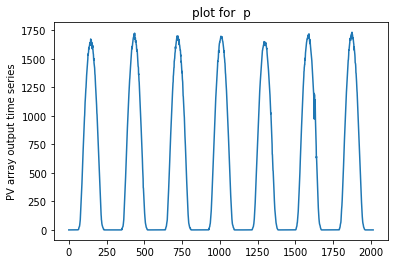
\includegraphics[width=\columnwidth]{p.png}
    \caption{PV array power plot}
    \label{}
\end{figure}
\item A company ’ XYZ ’ is constructing a road through a hilly area. The height
of the roadbed should be chosen in such a way that the total cost of construction
is minimized. The construction cost depends on the difference between height (h)
of the roadbed and the current elevation of the road (e). $h_i$ gives the height of
the roadbed at a distance $d_i$ meters down the road, where $d > 0$ is a given
discretization. The existing elevation at a point $d_i$ meters down the road is
given by $e_i$. 
\begin{align}
\vec{e} = 5\sin\displaystyle\frac{i}{3n\pi}+\sin\displaystyle\frac{i}{10n\pi} \nonumber
\end{align}
where i ranges from 1 to n, where n = 100.\\
The construction cost is mainly affected by the cuts(roadbed below existing
elevation) and fills(roadbed above existing elevation) present in the road. The
cut cost $\phi^\text{cut}$ and fill cost $\phi^\text{fill}$ are the linear functions of the difference between
the existing elevation of the road and height of the roadbed. The overall cost
(C) is a linear combination of the cut cost and fill cost. 
\begin{align}
& \vec{u} = \vec{h} -\vec{e} \nonumber\\
& (u)_+ = \text{max\{u,0\}} \nonumber\\
& (u)_- = \text{max\{-u,0\}} \nonumber\\
& \phi^\text{fill}(u) = 2(u)_+^2 + 30(u)_+ \nonumber\\
& \phi^\text{cut}(u) = 12(u)_-^2 + (u)_- \nonumber\\
&c= \phi^\text{cut}+\phi^\text{fill} \nonumber
\end{align}
The goal is to minimize $c$ subject to the following constraints.
\begin{itemize}
\item The maximum allowable road slope (first derivative $D^{(1)}$) is 0.08.
\item The maximum allowable curvature (second derivative $D^{(2)}$) is 0.025
\item The maximum allowable third derivative $D^{(3)}$ is 0.005
\end{itemize}
Formulate the optimization problem and verify the convexity of cut and fill functions by plotting for u in range $(1:0.1:10)$.  Plot $\vec{h}, \vec{e} \text{ and } \vec{u}$ for the optimal grading plan and report the associated cost.\\
\solution\\
Consider,
\begin{table}[H]
 \centering
 \resizebox{\columnwidth}{!}{
 \begin{tabular}{ |c|c|c| } 
 \hline
 \textbf{Description} & \textbf{Parameter} & \textbf{Value}  \\
 \hline
 Height of the road & $\vec{h}$ & $?$  \\ 
 \hline
Current elevation of the road & $\vec{e}$ & $ 5\sin\displaystyle\frac{i}{3n\pi}+\sin\displaystyle\frac{i}{10n\pi}$ \\
 \hline
 Discretization unit & d  &  1 \\ 
 \hline
Difference & $\vec{u} $ & $\vec{h}-\vec{e} $  \\
 \hline
 Filling height & $(u)_+$  & max\{u,0\}   \\
 \hline
 Cutting height & $(u)_-$   &max\{-u,0\}    \\
 \hline
 size of vectors & n & 100    \\
 \hline
 \end{tabular}}
 \caption{}
 \end{table}
 \begin{align}
& \vec{u} = \vec{h} -\vec{e} \nonumber\\
& (u)_+ = \text{max\{u,0\}} \nonumber\\
& (u)_- = \text{max\{-u,0\}} \nonumber\\
& \phi^\text{fill}(u) = 2(u)_+^2 + 30(u)_+ \nonumber\\
& \phi^\text{cut}(u) = 12(u)_-^2 + (u)_- \nonumber\\
&c= \phi^\text{cut}+\phi^\text{fill} \nonumber
\end{align}
 Objective function,
 \begin{align}
 z=\min_{\vec{h}} c
 \end{align}
 Constraints,
 \begin{align}
 & \displaystyle\frac{dh}{dn} \leq 0.08\\
 & \displaystyle\frac{d^2h}{dn^2} \leq 0.025\\
 & \displaystyle\frac{d^3h}{dn^3} \leq 0.005
 \end{align}
 CVXPY code,
 \begin{lstlisting}
https://github.com/gadepall/EE5606-optimization/codes/opt_6.py
\end{lstlisting}
 From CVXPY, the plots are as follows
 \begin{figure}[H]
	\centering
    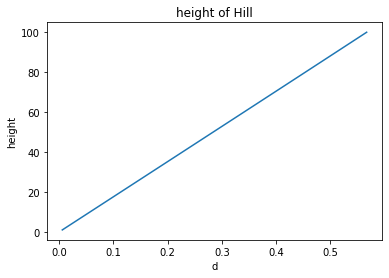
\includegraphics[width=\columnwidth]{h.png}
    \caption{Height plot}
    \label{}
\end{figure}
\begin{figure}[H]
	\centering
    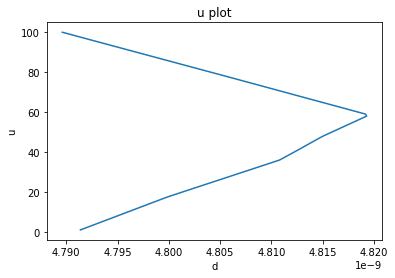
\includegraphics[width=\columnwidth]{u.png}
    \caption{U plot}
    \label{}
\end{figure}
\begin{figure}[H]
	\centering
    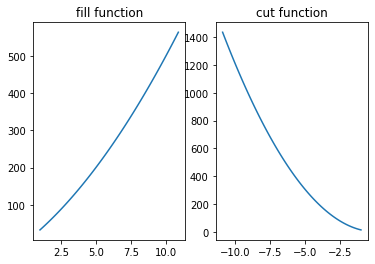
\includegraphics[width=\columnwidth]{fc.png}
    \caption{Fill and Cost plot}
    \label{}
\end{figure}
\begin{figure}[H]
	\centering
    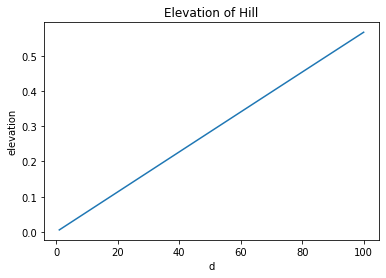
\includegraphics[width=\columnwidth]{e.png}
    \caption{Elevation plot}
    \label{}
\end{figure} 
\item Power Assignment in a Wireless Communication System: Consider a system with n transmitters, each with power $p_j \geq 0$, transmitting to n receivers. Let $G_{ij}\geq 0$ denote the path gain from transmitter j to receiver i. These path gains form the matrix $\vec{G} \in  \Re^{nxn}$.Each receiver is assigned to a transmitter such that the signal power at receiver i, $S_i=G_{ii}p_i$ and the interefence power at receiver i is $I_i =\Sigma_{k \neq i}G_{ik}p_k.$ Given a noise power $\sigma_{i}$  at each receiver, the SINR at receiver i, $\gamma_i=\displaystyle\frac{S_i}{I_i+\sigma_i}.$
The objective is to maximise the minimum SINR of the system under certain power constraints. These constraints are:
\begin{enumerate}
\item Each transmitter power$ p_j \leq P_j^{max}$.
\item If the transmitters are partitioned into m non-overlapping groups, $k_1,k_2....k_m,$ which share a common power supply with total power $P_l^{gp}, \Sigma_{k \in k_i} p_k \leq P_l^{gp}.$
\item There is a maximum power that each receiver can receive $P_i^{rc},\Sigma ^n_{k=1}G_{ik}p_k \leq P_i^{rc}$
\end{enumerate}
Formulate SINR as linear-fractional programming.\\
SINR maximization: We haven 5 transmitters, grouped into two groups : \{1,2\} and \{3,4,5\}. The maximum power for each transmitter is 3, the total  power limit for the first group is 4, and the total power limit for the second group is 6. The noise $\sigma$ is equal to 0.5 and the limit on total received power is 5 for each receiver. Finally, the path gain matrix is given by, \begin{align} \vec{G} =\myvec{1.0&0.1&0.2&0.1&0.0\\0.1&1.0&0.1&0.1&0.0\\0.2&0.1&2.0&0.2&0.2\\0.1&0.1&0.2&1.0&0.1\\0.0&0.0&0.2&0.1&1.0}\nonumber \end{align}
Find the transmitter powers $p_1,...,p_5$ that maximize the minimum SINR ratio overall receivers. Also report the maximum SINR value. Solving the problem to an accuracy of 0.05 (in SINR) is fine.\\
\solution \\
consider,
 \begin{table}[H]
 \centering
 \resizebox{\columnwidth}{!}{
 \begin{tabular}{ |c|c|c| } 
 \hline
 \textbf{Description} & \textbf{Parameter} & \textbf{Value}  \\
 \hline
 Powers of transmitter & $\vec{p}$ & $?$  \\ 
 \hline
Gain matrix & $\vec{G}$ & $\myvec{1.0&0.1&0.2&0.1&0.0\\0.1&1.0&0.1&0.1&0.0\\0.2&0.1&2.0&0.2&0.2\\0.1&0.1&0.2&1.0&0.1\\0.0&0.0&0.2&0.1&1.0} $ \\
 \hline
 Powers of receiver & $\vec{r}$  &  $\vec{Gp}$ \\ 
 \hline
noise & $\sigma $ & $\myvec{0.5\\0.5\\0.5\\0.5\\0.5} $  \\
 \hline
 no.of transmitters and receivers & n & 5    \\
 \hline
 \end{tabular}}
 \caption{}
 \end{table}
 However, since this is a quasiconvex objective function we cannot solve it directly using CVXPY. Instead we must use a bisection method. First we take the step of rewriting the objective, $\alpha =\gamma^{-1}$\\
 Objective function,
 \begin{align}
 z= \min_{\vec{p}} \alpha
 \end{align}
 Constraints,
 \begin{align}
 & \alpha \geq 0\\
 & \vec{p} \geq 0\\
 & \vec{p}\leq p^{max}\\
 &\vec{Gp} \leq \vec{p}^{rc}
 \end{align}
 Solving by CVXPY,\\
 CVXPY code,\\
 \begin{lstlisting}
https://github.com/gadepall/EE5606-optimization/codes/opt_7.py
\end{lstlisting}
\begin{align}
&z=0.7598 \nonumber\\
& \vec{p}= \myvec{0.51\\0.49\\0.32\\0.54\\0.47}\nonumber
\end{align}
\item Minimum time maneuver for a crane: Minimum time maneuver for a crane. A crane manipulates a load with mass $m > 0$ in two dimensions using two cables attached to the load. The cables maintain angles
 $\pm \theta$ with respect to vertical, as shown below,\\
 \begin{figure}[H]
	\centering
    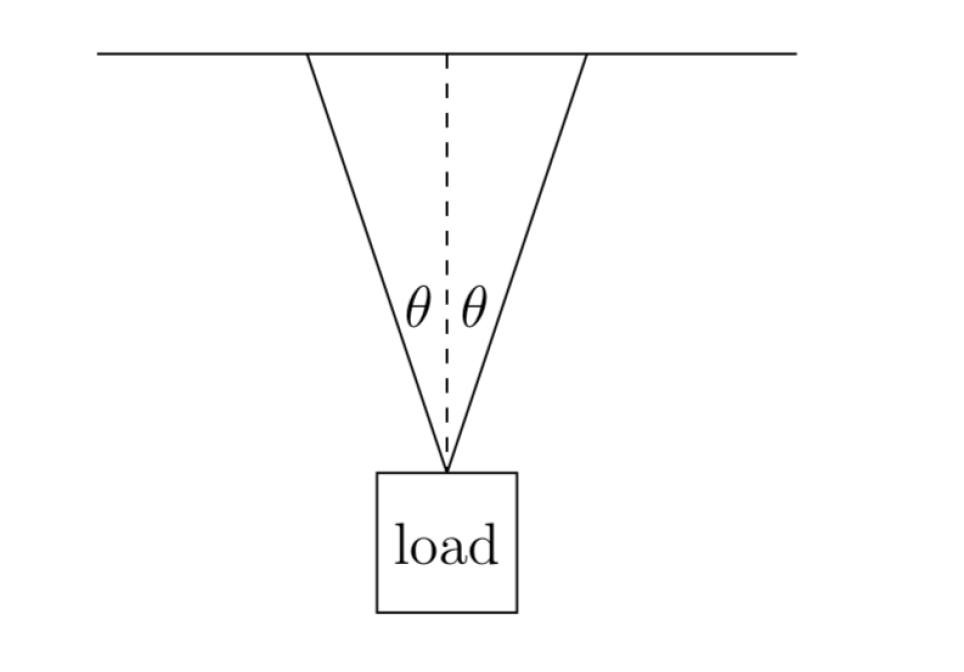
\includegraphics[width=\columnwidth]{load.png}
    \caption{Load}
    \label{}
\end{figure}
The (scalar) tensions $T^{left}$ and $T^{right}$ in the two cables are independently controllable,
from 0 up to a given maximum tension $T^{max}$. The total force on the load is
\begin{align}
F = T^{left}\myvec{-\sin\theta \\ \cos\theta}+T^{right}\myvec{\sin\theta \\ \cos\theta}+ mg
\end{align}
where g=9.8 $m/sec^2$, accelaration due to gravity.\\
The acceleration of the load is F/m. We approximate the motion of the load using
\begin{align}
&p_{i+1} = p_i + hv_i \nonumber\\ 
&v_{i+1} = v_i + (h/m)F_i, i = 1, 2, . . . , \nonumber
\end{align}
where $p_i \in \Re^2$ is the position of the load, $v_i \in \Re^2$ is the velocity of the load, and $F_i \in \Re^2$ is the force on the load, at time t = ih. Here $h > 0$ is a small (given) time step. The goal is to move the load, which is initially at rest at position $p_{init}$ to the position $p^{des}$, also at rest, in minimum time. In other words, we seek the smallest k for which
\begin{align}
p_1 = p^{init}, p_k = p^{des}, v_1 = v_k = (0, 0) \nonumber
\end{align}
is possible, subject to the constraints described above. \\
\begin{enumerate}
\item  Explain how to solve this problem using convex (or quasiconvex) optimization.
\item  Carry out the method of part (a) for the problem instance with
\begin{align}
&m = 0.1, \theta = 15\degree, T max = 2, p^{init} = (0, 0),\nonumber \\ & p^{des} = (10, 2), \text{ with time step } h = 0.1.\nonumber
\end{align}
\end{enumerate}
Report the minimum time k. Plot the tensions versus time, and the load trajectory, i.e., the points $p_1, . . . , p_k \text{ in } \Re^2$ . Does the load move along the line segment between $p^{init}$ and $p^{des}$ (i.e., the shortest path from $p^{init}$ and $p^{des}$)? Comment briefly.\\
\solution\\
CVXPY code,
\begin{lstlisting}
https://github.com/gadepall/EE5606-optimization/codes/opt_8.py
\end{lstlisting}
\item Suppose you manage n factories, each producing $s_i$ amount of goods for i = 1, 2, . . . , n. These goods
need to be shipped to m destinations, each having a demand $d_i$ for i = 1, 2, . . . , m, and our goal is to
move the goods from the factories to the destinations so as to satisfy the demand. However, there is a
cost associating to moving the goods: for moving a unit good from factory i to destination j, the cost
involved is $c_{ij}$ . Our goal is to decide the amount of quantities to be shipped from each factory to each
destination such that the demand is satisfied, and the overall cost is minimized. We assume that the
goods are divisible (so the quantity shipped does not have to be an integer), and that the shipping is
directly to the respective destinations (meaning there is no routing involved).
\begin{enumerate}
\item Formulate the problem above as an LP, and write a CVX/CVXPY code to compute the quantities
shipped.
\item Find the optimal transportation strategy for the following costs, supply and demands:
\end{enumerate}
\begin{table}[H]
 \centering
 \resizebox{\columnwidth}{!}{
 \begin{tabular}{ |c|c|c|c|c|c|c| } 
 \hline
 \textbf{Factory} & \textbf{$D_1$} & \textbf{$D_2$} & \textbf{$D_3$} & \textbf{$D_4$} & \textbf{$D_5$} & \textbf{Total Supply}  \\
 \hline
 Factory 1 & 8 & 6 & 19 &9 &8 & 40  \\ 
 \hline
 Factory 2 & 9 & 12 & 13 &7 &5 & 50  \\ 
 \hline
 Factory 3 & 14 & 9 & 16 &5 &2 & 45  \\ 
 \hline
 \textbf{Total demand} & 45 & 20 & 30 &30 &10 &   \\ 
 \hline
\end{tabular}}
 \caption{}
 \end{table}
\solution\\
consider,
 \begin{table}[H]
 \centering
 \resizebox{\columnwidth}{!}{
 \begin{tabular}{ |c|c|c| } 
 \hline
 \textbf{Description} & \textbf{Parameter} & \textbf{Value}  \\
 \hline
 No. of factories & n & 3  \\ 
 \hline
No. of destinations & m & 5 \\
 \hline
 Supply & $\vec{s}$  &  $\myvec{40\\50\\45}$ \\ 
 \hline
demand & $\vec{d} $ & $\myvec{45\\20\\30\\30\\10} $  \\
 \hline
 cost & $\vec{c} $ & $\myvec{8&6&10&9&8\\9&12&13&7&5\\14&9&16&5&2} $  \\
 \hline
 Amount of quantities to be shipped from each factory to each destination & $\vec{X}$ & $?$\\
 \hline
 \end{tabular}}
 \caption{}
 \end{table}
 Objective function,
 \begin{align}
 z=\min_{\vec{X}} \text{trace}(\vec{c}^\text{T}\vec{X})
 \end{align}
Constraints,
\begin{align}
& \vec{X}\vec{1} \preceq \vec{s}\\
& \vec{X}^T\vec{1} \succeq \vec{d}\\
& \vec{X} \succeq \vec{0}
\end{align}
solving by cvxpy\\
cvxpy code,
\begin{lstlisting}
https://github.com/gadepall/EE5606-optimization/codes/opt_9.py
\end{lstlisting}
Optimum value of z is 1025.
\item Consider the polynomial f(x) = $x^n$. We wish to approximate this polynomial with a degree n-1 polynomial $ a_0 + a_1x + a_2x^2 + . . . + a_{n-1}x^{n-1}$ on the interval [-1,1]. Consider partitioning the interval [-1,1] into 2N+1 equispaced points $-1 = x_{-N} , x_{-N+1}, . . . , x_{-1}, x_0 = 0, x_1, . . . , x_{N-1}, x_N = 1$.
Suppose we wish to pick the coefficients $a_i$ such that the following cost function is minimized:
\begin{align}
&\Sigma_{k=-N}^{N}(x_k^n-\Sigma_{i=0}^{n-1}a_ix_k^i)^2 \nonumber \\
&\Sigma_{k=-N}^{N}|x_k^n-\Sigma_{i=0}^{n-1}a_ix_k^i| \nonumber 
\end{align}
\begin{enumerate}
\item Formulate the problem of finding the coefficients $a_i$, and write a CVX/CVXPY code to compute the coefficients.
\item Find the coefficients for n = 5 n = 10, n = 20. Pick N to be large enough.
\end {enumerate}
\solution\\
consider,
\begin{align}
\vec{a}=\myvec{a_0\\.\\.\\a_{n-1}}
\end{align}
Objective function,
\begin{align}
&z_1= \min_{\vec{a}}\Sigma_{k=-N}^{N}(x_k^n-\Sigma_{i=0}^{n-1}a_ix_k^i)^2 \\
&z_2=\min_{\vec{a}}\Sigma_{k=-N}^{N}|x_k^n-\Sigma_{i=0}^{n-1}a_ix_k^i| 
\end{align}
Solving by using cvxpy.
cvxpy code,
\begin{lstlisting}
https://github.com/gadepall/EE5606-optimization/codes/opt_10.py
\end{lstlisting} 
\item Consider following program
\begin{align} 
\begin{aligned}
\min_{x_1,x_2} x_1^2+2x_2^2-x_1x_2-x1\\
\textrm{s.t.} x_1-2x_2\leq -2\\
   x_1+4x_2\leq -3  \\
   5x_1 -76 x_2 \leq 1\\
\end{aligned}
\end{align}
Solve the above problem using CVXPY\\
\solution\\
let,
\begin{align}
\vec{x}= \myvec{x_1\\x_2}
\end{align}
Objective function,
\begin{align}
z =\min_{x_1,x_2} x_1^2+2x_2^2-x_1x_2-x1\\
\end{align} 
Objective function can be equivalently written as,
\begin{align}
&z= \min_{\vec{x}}\vec{x^TAx}+\vec{b^Tx}\\
&\vec{A}=\myvec{1&-1/2\\-1/2&2}\\
&\vec{b}=\myvec{-1\\0}
\end{align}
constraints,
\begin{align}
&x_1-2x_2\leq -2\\
&x_1+4x_2\leq -3  \\
&5x_1 -76 x_2 \leq 1
\end{align}
Equivalent way of writting constraints,
\begin{align}
&\vec{Px} \preceq \vec{q}\\
&\vec{P}=\myvec{1&-2\\1&4\\5&-76}\\
&\vec{q}=\myvec{-2\\-3\\1}
\end{align}
Solving by cvxpy.\\
cvxpy code,
\begin{lstlisting}
https://github.com/gadepall/EE5606-optimization/codes/opt_11.py
\end{lstlisting} 
Optimum value of z = 7.44
\end{enumerate}
\end{document}


